\documentclass[12pt, twoside]{article}
\usepackage[letterpaper, margin=1in, headsep=0.5in]{geometry}
\usepackage[english]{babel}
\usepackage[utf8]{inputenc}
\usepackage{amsmath}
\usepackage{amsfonts}
\usepackage{amssymb}
\usepackage{tikz}
\usetikzlibrary{quotes, angles}
\usepackage{graphicx}
\usepackage{enumitem}
\usepackage{multicol}

\newif\ifmeta
\metatrue %print standards and topics tags

\title{Regents Geometry}
\author{Chris Huson}
\date{January 2022}

\usepackage{fancyhdr}
\pagestyle{fancy}
\fancyhf{}
\renewcommand{\headrulewidth}{0pt} % disable the underline of the header
\raggedbottom

\fancyhead[LE]{\thepage}
\fancyhead[RO]{\thepage \\ Name: \hspace{4cm} \,\\}
\fancyhead[LO]{BECA / Dr. Huson / Geometry 7 Similarity}

\begin{document}

\subsubsection*{7.3 Classwork: Scale applications \hfill CCSS.HSG.SRT.B.5}
\begin{enumerate}

\item Plot on the grid points representing these cities: Port-au-Prince is located at (3, -2) and Caracas is located at (6, -4). Washington DC is located at (3, 1) and New York City is located at (6, 2). Scale factor: 1 grid unit = 300 kilometers.

Find the distance between each pair of cities in grid units $and$ kilometers.

(a) New York City and Caracas.

(b) Port-au-Prince and Washington DC.

(c) Port-au-Prince and Caracas.

\begin{multicols}{2}
  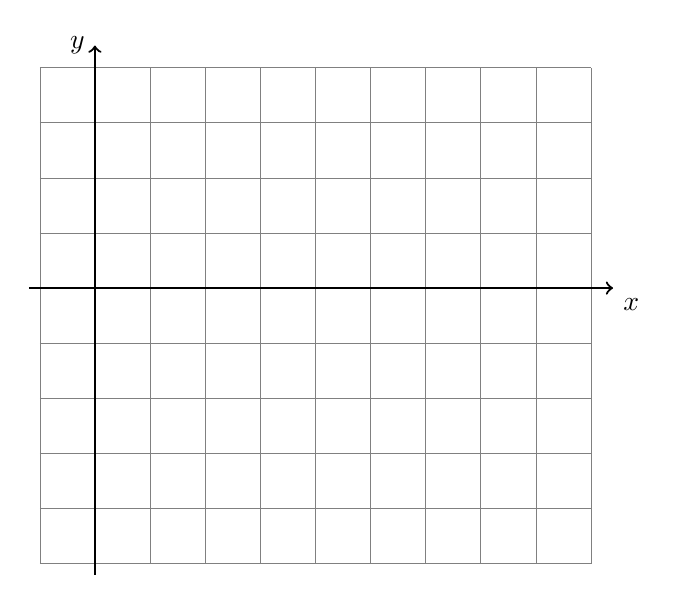
\begin{tikzpicture}[scale=.7]
    \draw [help lines] (-1,-5) grid (9,4);
    \draw [thick, ->] (-1.2,0) -- (9.4,0) node [below right] {$x$};
    \draw [thick, ->] (0,-5.2)--(0,4.4) node [left] {$y$};
  \end{tikzpicture}
\end{multicols}

\item Dr. Huson's classroom is 24.5 feet wide. A model of the classroom is 4 inches wide. What is the scale factor?\vspace{2cm}

\item A model of BECA has a scale of 1 in : 4 ft. If the real BECA is 332 feet wide then how wide is the model BECA?\vspace{2cm}

\item Boston and New York City are 147 cm apart from each other on a map. How far apart are the two cities in real life? The map's key tells you that 3 cm is 7 km.

\newpage
\item Triangle $HTS$, where $H$ = $Home$, is dilated with a scale factor of $k=1.75$ centered at $H$, yielding $\triangle HLC$, as shown. Given $HT$ = 7 km, $HS$ = 4.5 km, and $LC$ = 20 km.

(a) Student $A$ walks from school to the theatre and then walks to the library. How many kilometers did student $A$ walk?

(b) Student $B$ decides to walk from school to the cafe and then walk back home. How many kilometers did student $B$ walk?

\begin{flushright}
  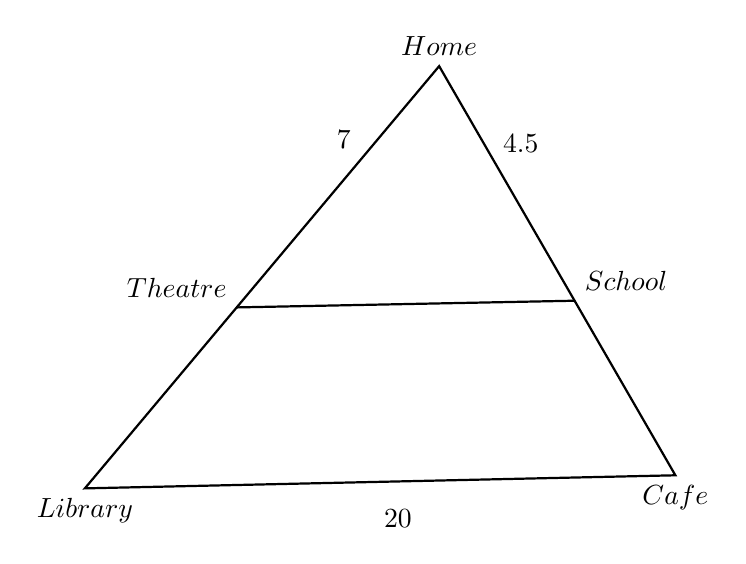
\begin{tikzpicture}[scale=0.8]
    \draw [thick]
    (0,0)node[above]{$Home$}--
    (-130:8.75)node[below]{$Library$}--
    (-60:7.5)node[below]{$Cafe$}--cycle;
    \draw [thick]
    (-130:5)node[above left]{$Theatre$}--
    (-60:4.3)node[above right]{$School$};
    \node at (-150:1.75)[below]{$7$};
    \node at (-55:1.5)[right]{$4.5$};
    \node at (-95:7.5)[above]{$20$};
  \end{tikzpicture}
\end{flushright} \vspace{0.5cm}

\item Reflect $\triangle ABC$ across the $y$-axis. Then, dilate $\triangle A'B'C'$ by a factor of k = 1.5 centered at the origin to produce $\triangle A''B''C''$. Plot and label the two triangles in the graph below.
\begin{center}
  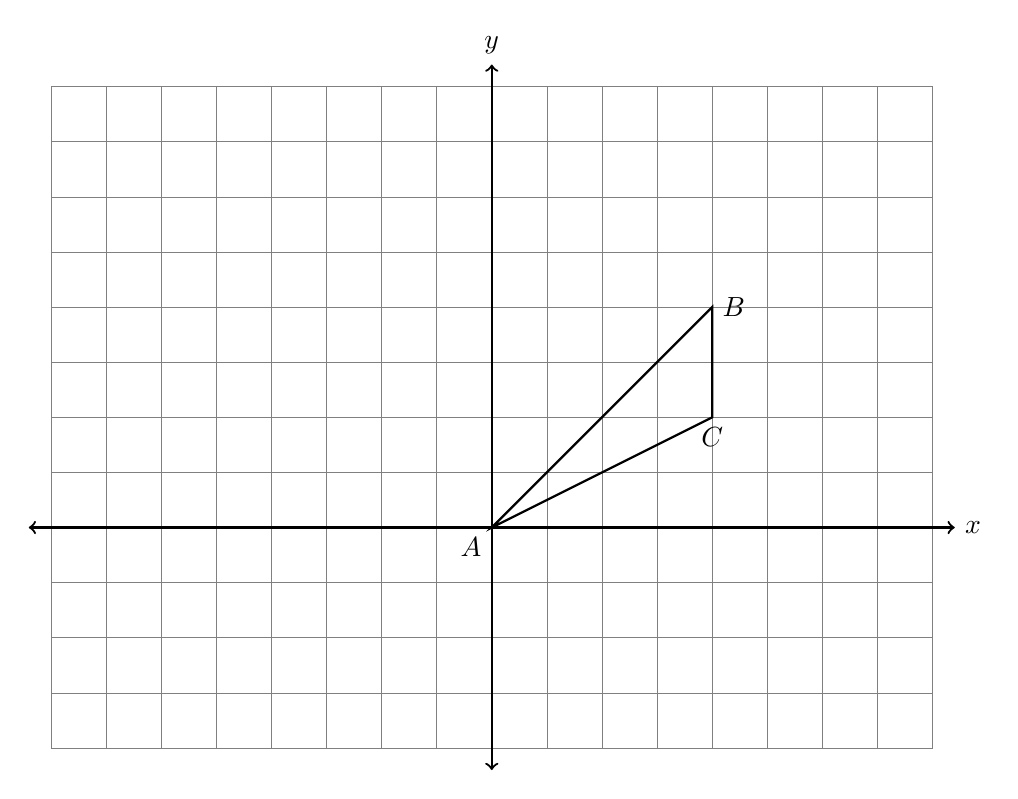
\begin{tikzpicture}[scale=.7]
    \draw [help lines] (-8,-4) grid (8,8);
    \draw [thick, <->] (-8.4,0) -- (8.4,0) node [right] {$x$};
    \draw [thick, <->] (0,-4.4)--(0,8.4) node [above] {$y$};
    \draw [thick]
      (0,0) node[below left] {$A$}--
      (4,4) node[right] {$B$}--
      (4,2) node[below] {$C$}--
      cycle;
  \end{tikzpicture}
\end{center}

\end{enumerate}
\end{document}
